\documentclass[12pt, a4paper, titlepage, table]{article}
\usepackage{pdfpages}
\usepackage[utf8]{inputenc}
\usepackage[T1]{fontenc}
\usepackage{titlesec}
\usepackage[french]{babel}
\usepackage{caption}
\usepackage{float}
\usepackage{graphicx}
\usepackage[inner=2cm, outer=2cm, top=2cm, bottom=2cm]{geometry}
\usepackage[T1]{fontenc}
\usepackage{times}
\usepackage{xr} 
\usepackage{multirow}
\usepackage{amsmath}
\usepackage{array}

\begin{document}
	\label{document}
	\title{Etude d'un MOOC}
	\author{Sébastien Mertès}
	\date{\today}
	\maketitle
	\renewcommand{\thesection}{\arabic{section}.}
	\renewcommand{\thesubsection}{\thesection\arabic{subsection}}
	\renewcommand{\tablename}{Tableau}
	\renewcommand{\abstractname}{Résumé}
	\captionsetup[table]{font={small}}
	\setlength{\parindent}{0pt}
	\captionsetup{labelfont=bf}
	\tableofcontents

\newpage	
\section{Principales variables utilisées}
Les principales variables utilisées dans cette analyse sont listées dans le Tableau 1. Il s'agit d'un jeu de données résultant d'une base d'apprenants à un MOOC et d'une autre base indiquant leurs parcours d'apprentissage par le suivi ou non des vidéos et le passage des quiz, de l'examen ou de la certification du MOOC. La formation du MOOC s'étend sur 5 semaines. L'indication des vidéos consultées est donnée par les variables S1 à S5 correspondant au numéro de la semaine  ainsi qu'aux quiz.
Le passage ou non de la certification et de l'examen est donné par les variables Exam.bin et Certif.bin. Le genre de l'apprenant est donnée par la variable Gender ainsi que son HDI par la variable Country\_HDI.

\begin{table}[H]
	\centering
	\fontsize{10}{12}\selectfont
	\begin{tabular}{|r|r|}
	\hline 
	\multicolumn{1}{|c|}{\textbf{Variable}}& 
	\multicolumn{1}{c|}{\textbf{Type}} \\
	\hline
   	Student\_ID&             int64\\      
   	Gender    &             object\\
	Country\_HDI&            object\\
	Exam.bin    &           bool\\   
	Assignment.bin&         int64\\  
	Quizz.1.bin&            int64 \\ 
	Quizz.2.bin&            int64 \\ 
	Quizz.3.bin&            int64 \\
	Quizz.4.bin&            int64 \\ 
	Quizz.5.bin&            int64 \\ 
	S1.L1      &            int64 \\ 
	S1.L2      &            int64 \\ 
	S1.L3      &            int64 \\ 
	S1.L4      &            int64 \\ 
	S1.L5      &            int64 \\
	S1.L6      &            int64 \\ 
	S2.L1      &            int64 \\ 
	S2.L2      &            int64 \\ 
	S2.L3      &            int64 \\ 
	S2.L4      &            int64 \\ 
	S2.L5      &            int64 \\ 
	S2.L6      &            int64 \\  
	S3.L1.1    &            int64 \\ 
	S3.L1.2    &            int64 \\ 
	S3.L2      &            int64 \\ 
	S3.L3      &            int64 \\ 
	S3.L4      &            int64 \\ 
	S3.L5      &            int64 \\ 
	S4.L1.1    &            int64 \\ 
	S4.L1.2    &            int64 \\ 
	S4.L2      &            int64 \\ 
	S4.L3      &            int64 \\ 
	S4.L4      &            int64 \\ 
	S4.L5      &           	int64 \\   
	S5.L1.1    &            int64 \\ 
	S5.L1.2    &            int64 \\ 
	S5.L2      &            int64 \\ 
	S5.L3      &            int64 \\ 
	S5.L4      &            int64 \\ 
	S5.L5      &            int64 \\ 
	Certif.bin &           bool  \\
	\hline
	\end{tabular}
	\caption{\textbf{Proportions des apprenants par type et par itération.}}
\end{table}  

\newpage
\section{Proportions des types d'apprenants par itération}
Le Tableau 2 montre la proportion de chacun des types d'apprenant par itération,  auditing, bystander, completer et disengaging par itération. Cela en fonction du nombre de vidéos vues, de quiz réalisés et du passage de l'examen ou de la certification ou non.

\begin{table}[H]
	\centering
	\fontsize{10}{12}\selectfont
	\begin{tabular}{|c|l|r|r|r|}
		\hline 
		\multicolumn{1}{|c|}{\textbf{Itération}} & 
		\multicolumn{1}{c|}{\textbf{Type}} &
		\multicolumn{1}{c|}{\textbf{Total/type}}&
		\multicolumn{1}{c|}{\textbf{Total/itération}}&
		\multicolumn{1}{c|}{\textbf{Pct/Type}}\\
		\hline
		1&	Auditing&		1207&	7965&	15.2\%\\
		1&	Bystander&		4285&	7965&	53.8\%\\
		1&	Completer&		20	&	7965&	0.3\%\\
		1&	Disengaging&	2453&	7965&	30.8\%\\
		2&	Auditing&		538	&	3702&	14.5\%\\
		2&	Bystander&		2168&	3702&	58.6\%\\
		2&	Completer&		876	&	3702&	23.7\%\\
		2&	Disengaging&	120	&	3702&	3.2\%\\
		3&	Auditing&		375	&	3515&	10.7\%\\
		3&	Bystander&		2238&	3515&	63.7\%\\
		3&	Completer&		832	&	3515&	23.7\%\\
		3&	Disengaging&	70	&	3515&	2.0\%\\
		\hline
	\end{tabular}
\caption{\textbf{Proportions des apprenants par type et par itération.}}
\end{table}

\section{Test d'indépendance du $\chi2$ entre le genre et l'HDI}

La Figure 1 représente les résidus du test d'indépendance fondé sur le chi2 entre le genre et l'HDI, afin de déterminer si il y un lien entre l'Human Development Index et le genre (homme ou femme).
Les cellules rouges indiquent que le modèle prédit (calculé) a sous-évalué la valeur observée puisque le résidu est positif. Et réciproquement, la couleur bleu indique un résidu négatif, indiquant que le modèle prédiction a sur-évalué la valeur observée. 

Le Tableau 3 indique le tableau de contingence des fréquences observées entre les variables catégorielles genre et HDI. Chacune comprenant respectivement 2 et 3 modalités. C'est à partir des valeurs de ce tableau que nous pouvons appliquer le test du $\chi^2$ et en déduire si les variables sont statistiquement indépendantes ou non.

\begin{table}[H]
	\centering
	\fontsize{10}{12}\selectfont
	\begin{tabular}{|c|l|r|r|r|}
		\hline 
		\multicolumn{1}{|c|}{\textbf{}} & 
		\multicolumn{1}{c|}{\textbf{B}} &
		\multicolumn{1}{c|}{\textbf{I}} &
		\multicolumn{1}{c|}{\textbf{TH}} \\
		\hline
 			Femme&	147&	233&	2545\\
 			Homme&	883&	432&	4711\\
		\hline
	\end{tabular}
\caption{\textbf{Tableau de contingence du genre et de l'HDI.}}
\end{table}

	\begin{figure}[H]
		\centering
		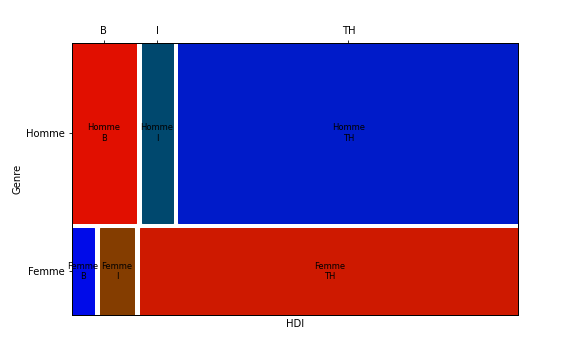
\includegraphics[width=1\textwidth]{../../graph/mosaic_contingence.png}
		\caption{\textbf{Mosaic des résidus du test du $\chi2$}}
	\end{figure}

La Figure 2, représente les résidus du modèle observé par rapport au modèle de prédiction. Nous observons que les écarts des résidus sont assez éloignés de la droite droite horizontale faisant référence à des écarts nuls entre les valeurs observées et calculées. Nous pouvons observer que le modèle de prédiction est assez éloigné du modèle observé.

	\begin{figure}[H]
		\centering
		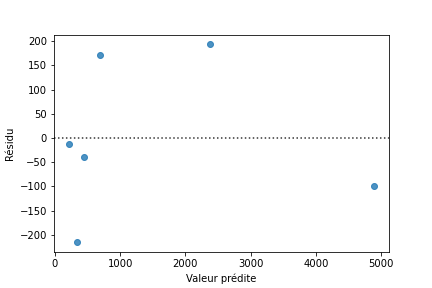
\includegraphics[width=0.7\textwidth]{../../graph/residus_chi2.png}
		\caption{\textbf{Résidus du test du $\chi2$}}
	\end{figure}


La formule de Cramer ci-dessous, mesure la force de l'association entre deux variables catégorielles.
\[ V = \sqrt{\frac{\chi^2}{n \cdot (\min(r, c) - 1)}} \]
V représente le coefficient de Cramer,  r est le nombre de modalités de la première variable et c est le nombre de modalités de la deuxième variable.
Nous allons appliquer cette formule aux variables précédentes indiquant le genre et HDI.
L'index HDI a 3 modalités (c) et le genre a 2 modalités (r), la valeur V est de 0,14.
Le tableau 4, résume les valeurs statistiques du test du $\chi^2$ et du V de Cramer.

\begin{table}[H]
	\centering
	\fontsize{12}{20}\selectfont
	\begin{tabular}{|l|r|}
		\hline  
		$\chi2$&	179.24\\
		p-value&	0\\
		V-Cramer&	0.14\\
		\hline
	\end{tabular}
	\caption{\textbf{Valeurs du $\chi2$ et du V de Cramer.}}
\end{table}

La p-value étant anormalement très proche de zéro et le V de Cramer étant faible, ces valeurs confirmeraient que le modèle de prédiction n'est pas fidèle au modèle observé. En conséquence, en déduire que la dépendance entre le genre et l'index HDI est statistiquement significative (p-value < 5 \%) et que celle-ci est très faible (V proche de 0), serait erronée. Nous pouvons donc envisager qu'il n'y a pas de lien entre le genre et l'index HDI. Cela confirmerait l'hypothèse d'indépendance de départ.

\section{Modèle linéaire, tests non paramétriques}
\subsection{Tests statistiques entre le nombre de vidéos visionnées et le genre}
Après l'index HDI, intéressons-nous aux nombres de vidéos vues par rapport au genre. Le figure 3 montre le nombre moyen de visionnage pour les femmes et les hommes. Son observation montrerait qu'en moyenne il y aurait une très faible différence entre les hommes et les femmes sur le nombre de vidéos vues. 

	\begin{figure}[H]
		\centering
		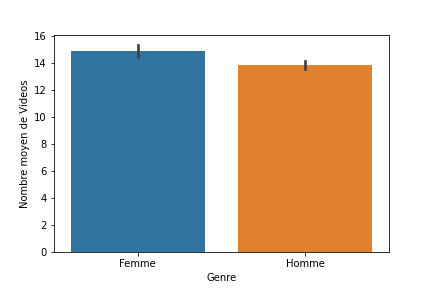
\includegraphics[width=0.7\textwidth]{../../graph/mean_video.png}
		\caption{\textbf{Moyenne des vidéos vues par genre.}}
	\end{figure}

L'hypothèse de départ (H0) est qu'il n'y a aucune différence sur le nombre de vidéos vues entre les hommes et les femmes. La figure 4, montre la distribution du nombre de vidéo pour les hommes et les femmes. Nous pouvons constater que la distribution des données ne ressemble pas à une distribution normale.

	\begin{figure}[H]
		\centering
		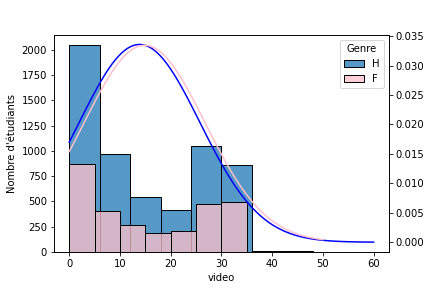
\includegraphics[width=0.8\textwidth]{../../graph/distribution_video.png}
		\caption{\textbf{Distribution du nombre de vidéos par genre.}}
	\end{figure}

La Figure 5, compare les quantiles de la distribution des vidéos des 2 modalités homme et femme afin de déterminer graphiquement si la distribution est normale. Nous observons également que la distribution observée ne suit pas la distribution théorique normale. Cela confirmerait l'hypothèse que la distribution observée n'est pas gaussienne.


  	\begin{figure}[H]
  		\centering
  		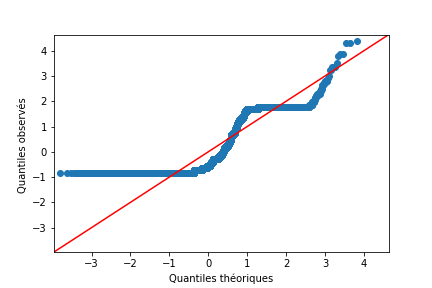
\includegraphics[width=0.8\textwidth]{../../graph/distribution_video3.png}
  		\caption{\textbf{Normalité de la distribution du nombre de vidéos selon le genre.}}
  	\end{figure}
  
La taille des échantillons étant conséquente nous pouvons appliquer le test de   Kolmogrov-Smirnov (KS) pour vérifier la normalité des données. L'hypothèse de départ (H0) est que la distribution est gaussienne.
Le résultat de ce test donnant une valeur de 0 de la p-value, la normalité n'est pas statistiquement significative et conclure qu'il est fortement probable que celle-ci ne l'est pas.   
En conséquence des différents tests de normalité de la distribution des données du nombre de vidéos pour les 2 modalités homme et femme, il est indiqué de procéder à un test non paramétrique afin de déterminer si il y a une différence sur le nombre de vidéos visonnées entre hommes et femmes. 

Le Tableau 5 affiche les valeurs du test non paramétrique de Mann-Whitney U. Les résultats, montreraient que l'hypothèse d'absence de différence entre le nombre de vidéos vues et le genre n'est pas statistiquement significatif (p-value < 5\%). Il existerait donc une différence sur le nombre de vidéos vues entre les hommes et les femmes.

\begin{table}[H]
	\centering
	\fontsize{12}{20}\selectfont
	\begin{tabular}{|c|c|}
		\hline
		\multicolumn{2}{|c|}{\textbf{Test Mann-Whitney U}}\\ 
		\hline 
		statistic& 8200580.5\\
		p-value& 0\\
		\hline
	\end{tabular}
\caption{\textbf{Test non paramétriques.}}
\end{table}

\subsection{Tests statistiques entre le nombre de vidéos visionnées et le nombre de quiz réalisés.}
Afin de déterminer quel test de corrélation il faut appliquer, il est nécessaire de savoir si les données suivent une distribution normale ou non. La Figure 6, montre que la distribution observée ne suit pas la distribution théorique normale en rouge.
En l'absence de normalité de distribution, on utilisera un test de Spearman afin de tester la corrélation entre le nombre de vidéos visionnées et le nombre de quiz. 

\begin{figure}[H]
	\centering
	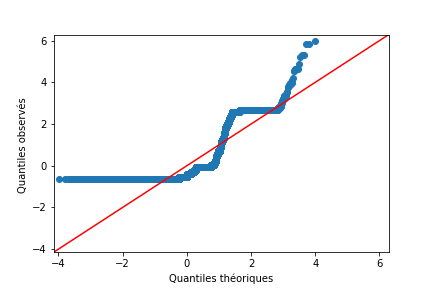
\includegraphics[width=0.8\textwidth]{../../graph/distribution_video4.png}
	\caption{\textbf{Normalité de la distribution du nombre de vidéos selon le nombre de quiz.}}
\end{figure}

Selon les résultats obtenus dans le Tableau 6 du test de Spearman, il y aurait une forte corrélation (0.8) entre le nombre de vidéos vues et le nombre de quiz réalisés par un étudiant. La corrélation observée est statistiquement significative (p-value=0).
\begin{table}[H]
	\centering
	\fontsize{12}{20}\selectfont
	\begin{tabular}{|c|c|}
		\hline
		\multicolumn{2}{|c|}{\textbf{Test de Spearman}}\\ 
		\hline 
		statistic& 0.80\\
		p-value& 0\\
		\hline
	\end{tabular}
	\caption{\textbf{Test de corrélation.}}
\end{table}

La Figure 7, représente le scatter plot des valeurs observées et le modèle de régression linéaire par la droite tracée en rouge entre le nombre de quiz effectués et le nombre de vidéos visionnées. Cependant, le modèle linéaire théorique extrapolerait un nombre de quiz bien supérieur à 10 au delà de 60 vidéos visionnées alors que la tendance des valeurs observées suggère un plafonnement du nombre de quiz à 10. La fonction linéaire ne serait pas le modèle le plus adapté en comparaison aux données réelles.

\begin{figure}[H]
	\centering
	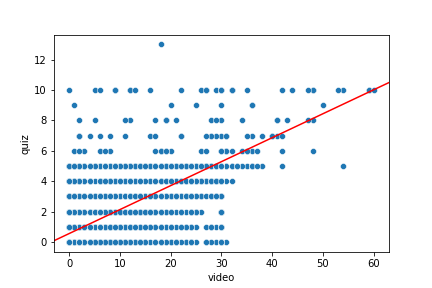
\includegraphics[width=0.8\textwidth]{../../graph/scatter2_regression.png}
	\caption{\textbf{valeurs observées (bleu) et modèle de régression linéaire (rouge).}}
\end{figure}

Le Tableau 7 indique les résultats du modèle de régression à la variable dépendante quiz et à la variable explicative quiz. Le $R^2$ à 0.64, indiquerait que les valeurs prédites représenteraient 64\% des valeurs observées. 
Selon les résultats du tableau 8, la p-value étant de 0, il y aurait statistiquement un lien sur le nombre de vidéos vues et le nombre de quiz effectués. Selon le modèle théorique, il y aurait presque 5 fois moins de quiz effectués que de nombre de vidéos visionnées.

\begin{table}[H]
	\centering
	\fontsize{12}{20}\selectfont
	\begin{tabular}{|ll|ll|}
		\hline
			Dep. Variable:&	quiz&	R-squared:&	0.646\\
			Model:&	OLS&	Adj. R-squared:&	0.646\\
			Method:&	Least Squares&	F-statistic:&	2.653e+04\\
			No. Observations:&	14557&	AIC:&	4.997e+04\\
			Df Residuals:&	14555&	BIC:&	4.998e+04\\
		\hline
	\end{tabular}
\caption{\textbf{Résultats de modèle de régression linéaire (video vs squiz).}}
\end{table}
	
	
\begin{table}[H]
	\centering
	\fontsize{12}{20}\selectfont
	\begin{tabular}{|l|r|r|r|r|}
		\hline
			\multicolumn{1}{|c|}{\textbf{}}&
			\multicolumn{1}{c|}{\textbf{coef}}&
			\multicolumn{1}{c|}{\textbf{std err}}&
			\multicolumn{1}{c|}{\textbf{t}}&
			\multicolumn{1}{c|}{\textbf{p-value}}\\	
		\hline
		\textbf{Intercept}&	0.5652&	0.014&	39.183&	0***\\
		\textbf{video}&	0.1575&	0.001&	162.896&	0***\\
		\hline
\end{tabular}
\caption{\textbf{Modèle de régression-vidéo vs quiz.}}
\end{table}

	\subsection{ANOVA sans intéraction sur le nombre de vidéos selon le genre et l'HDI}
	
	Dans le Tableau 9, le degrés de liberté (df) pour le genre est de 1 car la variable contient 2 modalités (homme et femme).
	\[ df = n[mod] - 1 \]
	Avec n représentant le nombre de modalités (mod) des variables, Genre et New\_HDI.
	La variable Genre comporte 2 modalités (homme et femme) donc le df est de 1. La variable New\_HDI comporte 3 modalités (TH, I, B), donc le df est de 2.
	  
	\begin{table}[H]
		\centering
		\fontsize{12}{20}\selectfont
		\begin{tabular}{|l|r|r|r|r|r|}
			\hline
					\multicolumn{1}{|c|}{\textbf{}}&
					\multicolumn{1}{c|}{\textbf{df}}&
					\multicolumn{1}{c|}{\textbf{sum\_sq}}&
					\multicolumn{1}{c|}{\textbf{mean\_sq}}&
					\multicolumn{1}{c|}{\textbf{F}}&
					\multicolumn{1}{c|}{\textbf{PR(>F)}}\\
			\hline
				\textbf{C(Genre)}&	1&	1554.89&	1554.9&	11.43&	0***\\
				\textbf{C(New\_HDI)}&	2&	70714.83&	35357.41&	260.08&	0***\\
				\textbf{Residual}&	8861.0&	1204643&	135.95&		&		\\
			\hline
		\end{tabular}
		\caption{\textbf{Table d'ANOVA sans interaction - vidéo vs genre et HDI.}}
	\end{table}

	La sortie du modèle de régression du Tableau 10, décrit la relation statistique entre les variables explicatives, Genre et New\_HDI avec la variable de réponse video. L'équation linéaire résultante du modèle de régression est de la forme : 
	\[ Y=\beta0 + \beta1X1 + \beta2X2 + \beta3X3 \]
	
	Avec :\\
	$Y =$ nombre de vidéos visionnées\\
	$\beta0 = 7.0011$\\
	$\beta1 = 0.0959 : X1 = Genre(homme)$\\
	$\beta2 = 4.6774 : X2 = New\_HDI(I)$\\
	$\beta3 = 8.6728 : X3 = New\_HDI(TH)$\\
	
	Le groupe des femmes et l'index B de l'HDI sont utilisés comme référence (intercept) dans le modèle.
	En effet, le coefficient $\beta0$ correspond au nombre moyen de vidéos visionnées par les femmes dans la catégorie B. Les catégories TH ($X3$) et I ($X2$), sont comparées à l'index B.
	Ainsi, le nombre de vidéos visionnées est significativement indépendant des hommes ($X1$) par rapport aux femmes (p-value de 72 \%), contrairement aux HDI I et TH par rapport à l'index B
	
	\begin{table}[H]
		\centering
		\fontsize{12}{20}\selectfont
		\begin{tabular}{|l|r|r|r|r|}
			\hline
			\multicolumn{1}{|c|}{\textbf{}}&
			\multicolumn{1}{c|}{\textbf{coef}}&
			\multicolumn{1}{c|}{\textbf{std err}}&
			\multicolumn{1}{c|}{\textbf{t}}&
			\multicolumn{1}{c|}{\textbf{p-value}}\\	
			\hline
			\textbf{Intercept}&			7.0011&		0.432&	16.211&	0***\\	
			\textbf{C(Genre)[T.Homme]}&	-0.0959&	0.267&	-0.360&	0.719\\
			\textbf{C(New\_HDI)[T.I]}&	4.6774&		0.586&	7.979&	0***\\
			\textbf{C(New\_HDI)[T.TH]}&	8.6728&		0.395&	21.937&	0***\\
			\hline
		\end{tabular}
		\caption{\textbf{Modèle de régression-vidéo vs genre et HDI (sans interaction).}}
	\end{table}	

	\subsection{ANOVA avec interactions sur le nombre de vidéos selon le genre et l'HDI}	
	Dans le Tableau 11, l'interaction entre le genre et les catégories de l'HDI ont été ajoutées. La différence sur le nombre de vidéos visionnée par les hommes  par rapport aux femmes est toujours significativement négligeable (p-value de 65\%). Les femmes au contraire ont un effet significatif (p-value nulle) ainsi que l'HDI I et TH (p-value = 2.5\%) par rapport à l'index de référence B. Le nombre de videos visionnées dépend significativement des hommes de l'index I par rapport aux femmes de l'index B, contrairement aux hommes de l'HDI TH (p-value de 86 \%). 
	
	\begin{table}[H]
		\centering
		\fontsize{12}{20}\selectfont
		\begin{tabular}{|l|r|r|r|r|}
			\hline
			\multicolumn{1}{|c|}{\textbf{}}&
			\multicolumn{1}{c|}{\textbf{coef}}&
			\multicolumn{1}{c|}{\textbf{std err}}&
			\multicolumn{1}{c|}{\textbf{t}}&
			\multicolumn{1}{c|}{\textbf{p-value}}\\	
			\hline
				\textbf{Intercept}&			7.3310&			0.968&	7.573&	0***\\
				\textbf{C(Genre)[T.Homme]}&	-0.4810&		1.046&	-0.460&	0.646\\	
				\textbf{C(New\_HDI)[T.I]}&	2.7733&			1.236&	2.244&	0.025*\\	
				\textbf{C(New\_HDI)[T.TH]}&	8.4673&			0.995&	8.506&	0***\\	
				\textbf{C(Genre)[T.Homme]:C(New\_HDI)[T.I]}&	2.8032&	1.415&	1.982&	0.048*\\
				\textbf{C(Genre)[T.Homme]:C(New\_HDI)[T.TH]}&	0.1933&	1.085&	0.178&	0.859\\
			\hline
		\end{tabular}
	\caption{\textbf{Modèle de régression-vidéo vs genre et HDI (avec interaction).}}
\end{table}
	
	D'après le Tableau 12, le nombre de videos visionnés dépend significativement du genre (p-value = 0) et de l'HDI (p-value = 0), ainsi que du genre par rapport à l'HDI (p-value = 3\%).
	
	\begin{table}[H]
		\centering
		\fontsize{12}{20}\selectfont
		\begin{tabular}{|l|r|r|r|r|r|}
			\hline
			\multicolumn{1}{|c|}{\textbf{}}&
			\multicolumn{1}{c|}{\textbf{df}}&
			\multicolumn{1}{c|}{\textbf{sum\_sq}}&
			\multicolumn{1}{c|}{\textbf{mean\_sq}}&
			\multicolumn{1}{c|}{\textbf{F}}&
			\multicolumn{1}{c|}{\textbf{PR(>F)}}\\
			\hline
				\textbf{C(Genre)}&	1&	1554.89&	1554.89&	11.44&	0***\\
				\textbf{C(New\_HDI)}&	2&	70714.83&	35357.41&	260.22&	0***\\
				\textbf{C(Genre):C(New\_HDI)}&2&	954.15&	477.076535&	3.511225&0.03*\\
				\textbf{Residual}&	8859&	1203688&	135.87&	&	\\
			\hline
		\end{tabular}
	\caption{\textbf{Table d'ANOVA avec interaction - video vs genre et HDI.}}
\end{table}


\section{Régression logistic}
Nous allons maintenant utiliser une régression logistic afin de mesurer statistiquement la dépendance de l'obtention de l'examen et/ou de la certication entre le genre et l'HDI.


\begin{table}[H]
	\centering
	\fontsize{12}{20}\selectfont
	\begin{tabular}{|l|l|r|r|r|}
		\hline
		\multicolumn{1}{|c|}{\textbf{Type}}&
		\multicolumn{1}{c|}{\textbf{Coef}}&
		\multicolumn{1}{c|}{\textbf{MOOC V1}}&
		\multicolumn{1}{c|}{\textbf{MOOC V2}}&
		\multicolumn{1}{c|}{\textbf{MOOC V3}}\\
		\hline
		odds-ratio& Réf (homme/HDI I)&			0&		0.44&	1.27\\
		&			Gender[T.une femme]&1.87&		1.02&	0.81\\
		&			New\_HDI[T.I]&		0&		1.05&	1.06\\
		&			New\_HDI[T.TH]&		1.25&		1.56&	0.84\\
		\hline
		p-value&	Réf (homme/HDI I)	&		0***&		0***	&0.16\\
		&			Gender[T.une femme]&0.17&		0.83&	0.05\\
		&			New\_HDI[T.I]&		1&		0.85&	0.81\\
		&			New\_HDI[T.TH]&		0.77&		0***&	0.31\\
		\hline
		CI&			Réf (homme/HDI I)&			[-7.31, -4.51]&	[-1.11, -0.53]&	[-0.09, 0.57]\\
		&			Gender[T.une femme]&[-0.27, 1.52]&	[-0.16, 0.2]&	[-0.42, 0.0]\\
		&			New\_HDI[T.I]&		[-34263.64, 34221.85]&	[-0.42, 0.51]&	[-0.43, 0.55]\\
		&			New\_HDI[T.TH]&		[-1.26, 1.71]&	[0.14, 0.75]&	[-0.53, 0.17]\\
		\hline
	\end{tabular}
		\caption{\textbf{Examen - odds-ration, p-value et intervalle de confiance (CI).}}
		
\end{table}

\end{document}